\thispagestyle{empty} %Oculta o numero da primeira pagina do capitulo
\vspace{3ex}


\chapter{Estudo de viabilidade do método KPLS na predição de vida em fadiga.}

\section{Introdução}
% O método KPLS (Kriging e médios quadrados parciais), quando usado na predição de séries temporais de tensão, pode resultar em boas aproximações a baixos custos computacionais.

Neste segmento estuda-se os impactos da utilização do método KPLS (\emph{Kriging model and partial least squares}) na predição de séries temporais de tensão para aplicação no estudo da vida em fadiga dos risers. No caso deste estudo, a análise é feita a partir das tensões externas de Von Mises desenvolvidas a partir do software Anflex do CENPES/PETROBRAS. O caso analisado consiste em um longo \emph{riser} com flutuadores (Fig. \ref{figure.1}) que tornam flutuante parte da estrutura submersa (configuração \emph{lazy-wave}). 

\begin{figure}[!ht]
    \centering
    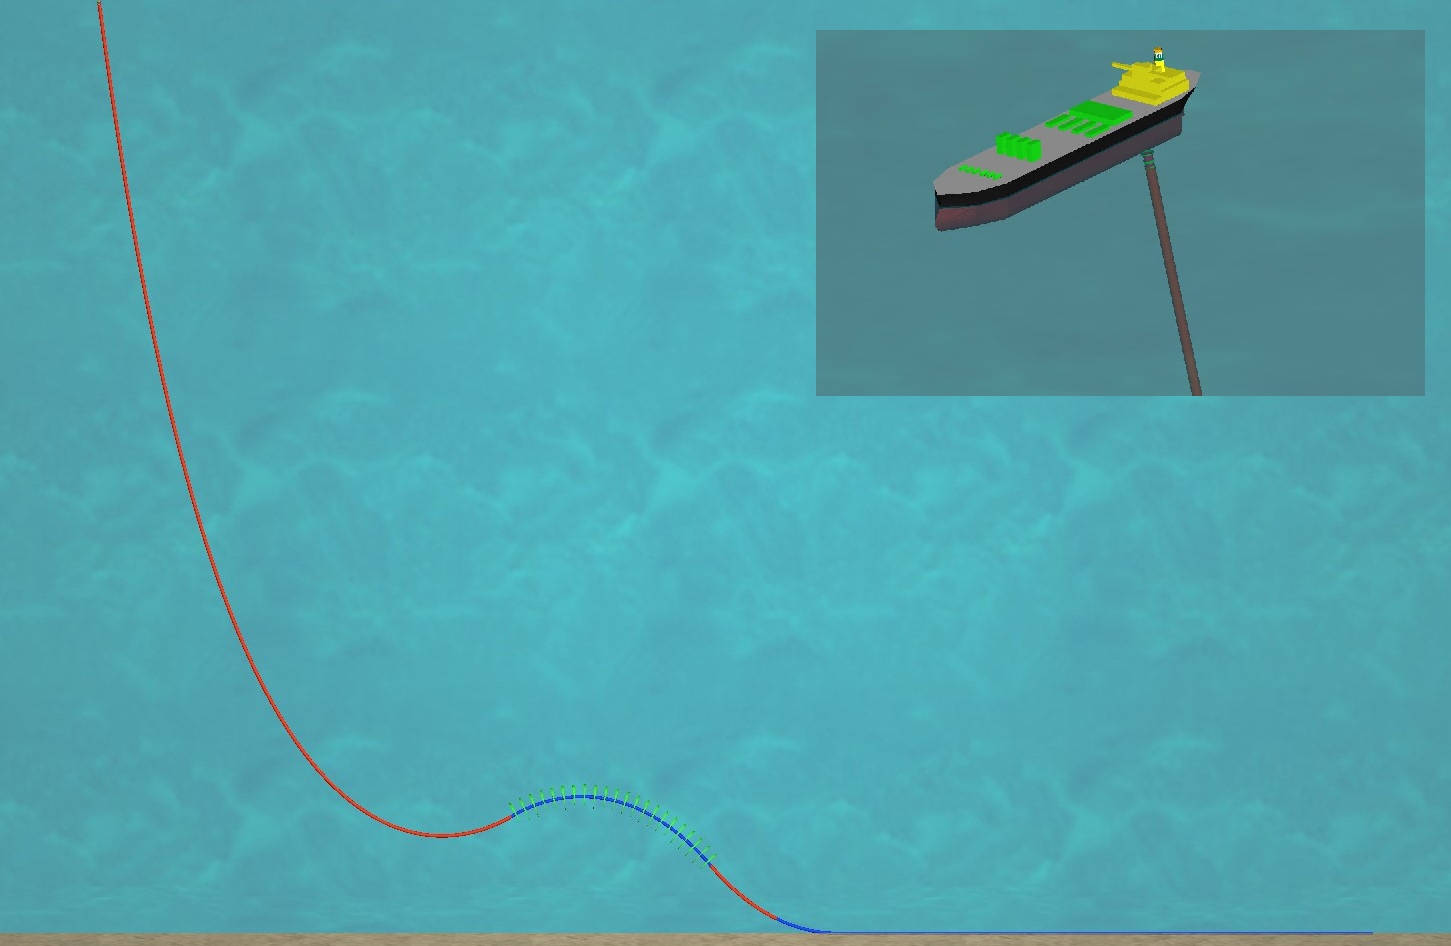
\includegraphics[width=0.5\linewidth , trim = {40mm 0mm 30mm 5mm} , clip]{felipe/fig_felipe/caso_estudado.jpg}
    \caption{Configuração \emph{lazy-wave}, onde o estudo foi desenvolvido.}
    \label{figure.1}
\end{figure}

O segmento flutuante (denominado região de SAG/HOG) tem o objetivo de atenuar os carregamentos advindos dos deslocamentos da estrutura flutuante no segmento do \emph{riser} em contato com o leito marinho. Seus efeitos podem ser observados no andamento deste estudo ao causar notável influencia na vida em fadiga dos elementos próximos. 

A biblioteca SMT foi utilizada para aplicação do método KPLS. Este pacote possui muitas ferramentas de metamodelo também aplicadas neste projeto \cite{BOUHLEL2019}.

Dessa forma, tem-se o intúito de se aplicar o método \emph{RainFlow} e o método de Goodman modificado para determinação da vida em fadiga a partir das séries de tensões externas de Von Mises advindas das simulações feitas no Anflex. O método KPLS é utilizado para predição parcial destas séries e então se calcula a vida em fadiga destas séries parcialmente ajustadas. Ao comparar-se os resultados observou-se boa conformidade, o que levanta boas oportunidades de otimização ao tornar facultativo o desenvolvimento de uma simulação completa para este tipo de análise. 

\section{Metodologia}

Para o estudo da vida em fadiga se utilizou o método \emph{RainFlow} e o método de Goodman modificado, enquanto que o método utilizado para se prever as séries temporais foi o \emph{KPLS}. 

\subsection{Método RainFlow}\label{rainflow}
Desenvolvido em 1968 por Tatsuo Endo e M. Matsuishi segundo \cite{dowling2007}, o método \emph{Rainflow} tem o objetivo de identificar os ciclos individuais de carregamento. Estas informações, ao se analisar séries temporais periódicas, podem ser usadas no desenvolvimento da vida em fadiga da estrutura analisada, isto é, o número de ciclos que o objeto de estudo aguentará antes de uma fratura devido à fadiga ocorrer. Ele foi desenvolvido com inspiração nos \emph{pagodes}, que são construções de arquitetura asiática muito utilizados como templos budistas (Fig.\ref{pagode}) em países como o Japão, China e as Coreias. 

\begin{figure}[!ht]
    \centering
    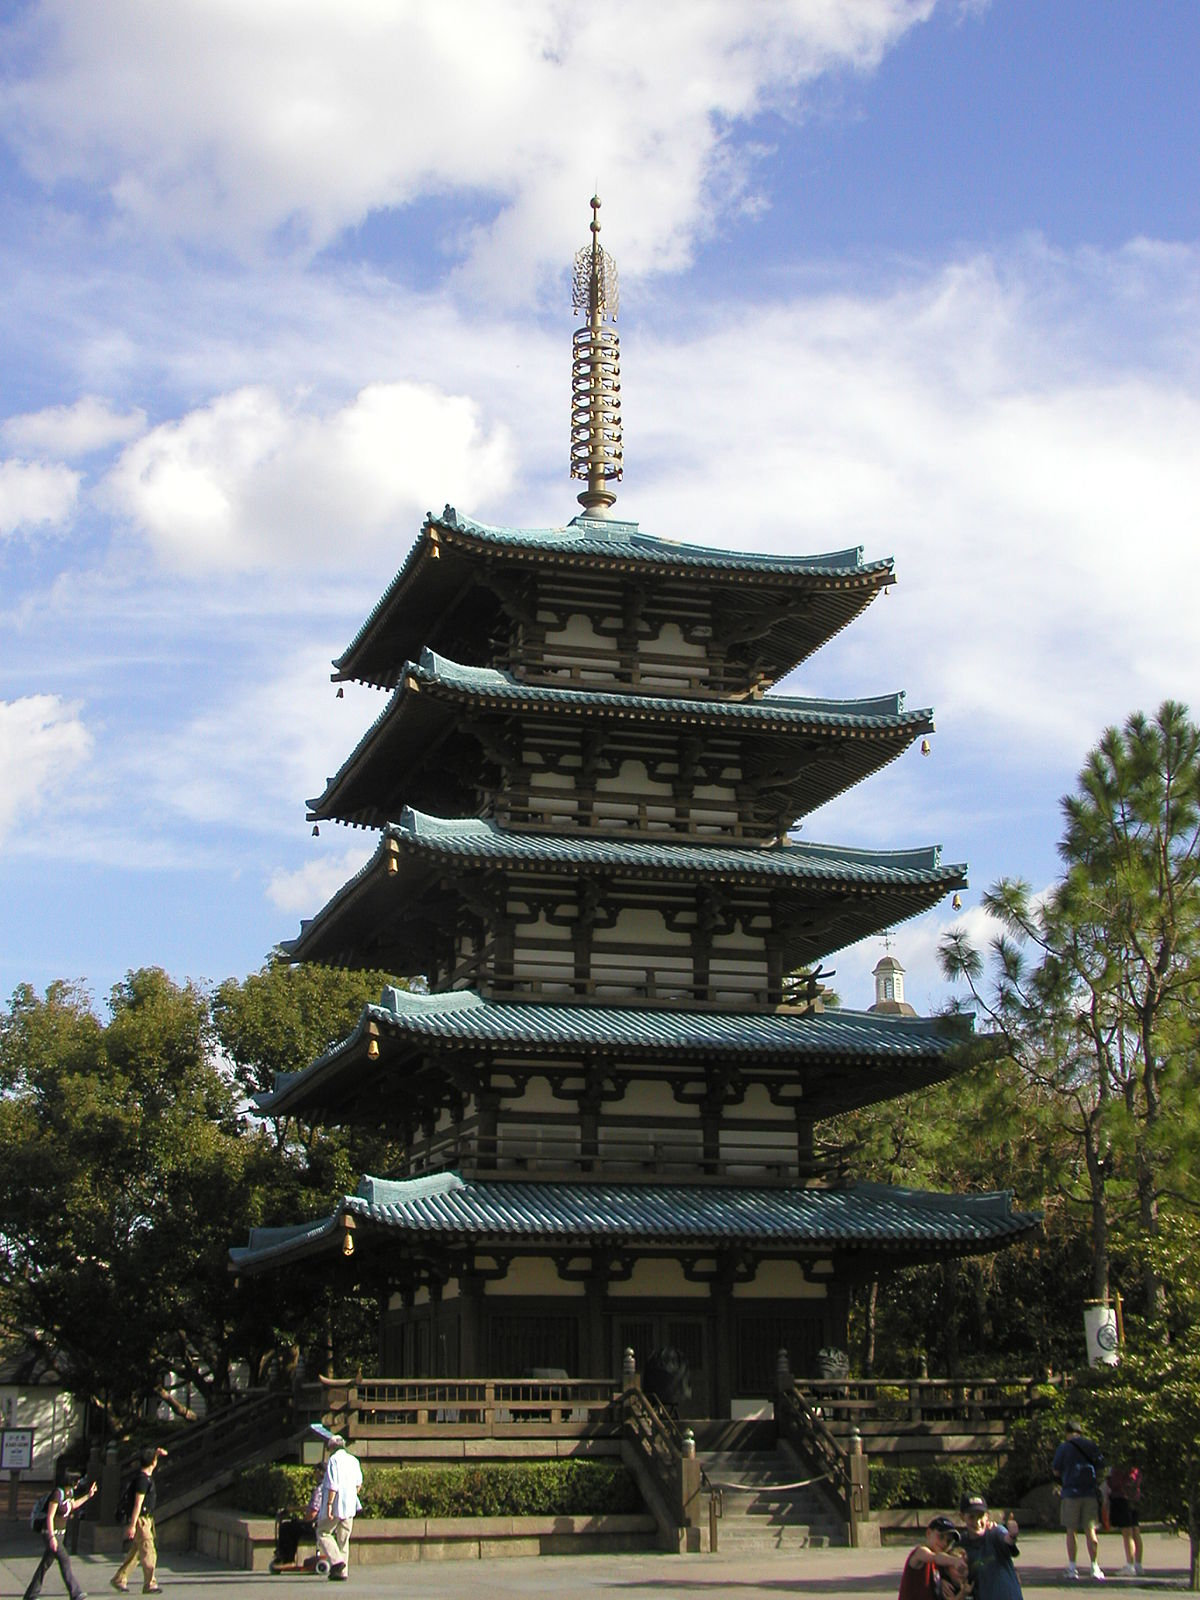
\includegraphics[width=0.25\linewidth , trim = {0mm 0mm 0mm 0mm} , clip]{felipe/fig_felipe/pagode.jpg}
    \caption{Pagode asiático.}
    \label{pagode}
\end{figure}

O método se baseia na analogia de um dia de chuva sobre um \emph{pagode}. Ao deixar um dos telhados a água cai verticalmente, podendo ou não tocar os telhados subsequentes. Tocar ou não o andar de baixo tem carácter classificatório sobre um ponto de vista de ciclos de carregamento. Ao se analisar três pontos em uma série temporal (pico, vale e pico) e se imaginar a situação descrita pela analogia, se a água que deixa o primeiro pico não tocar o segundo não há um ciclo de carregamento. Se, por outro lado, tocar, tem-se então identificado um ciclo de carregamento (Fig.\ref{rain_flow_1}). O mesmo pensamento pode ser aplicado em situações de vale, pico e vale.

\begin{figure}[!ht]
    \centering
    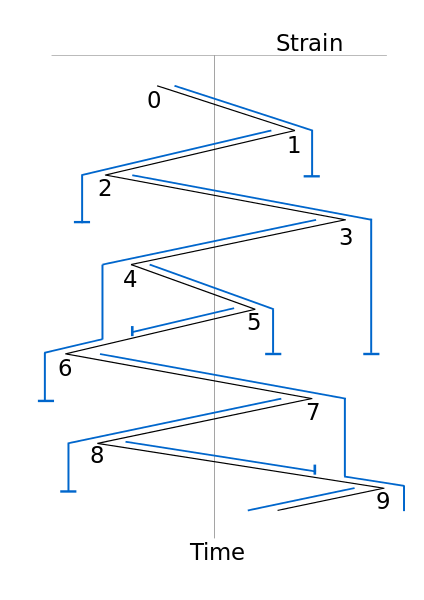
\includegraphics[width=0.4\linewidth, angle=90 , trim = {0mm 0mm 0mm 0mm} , clip]{felipe/fig_felipe/rainflow_1.png}
    \caption{Analogia do \emph{pagode} aplicada em um exemplo matemático.}
    \label{rain_flow_1}
\end{figure}

Dessa forma é oportuno pontuar o método com rigor matemático. A análise \emph{Rainflow} é aplicada a conjuntos de três pontos ($X$ , $Y$ e $Z$). Assim, quando $\left|\Delta_{YZ} \right|$ é maior ou igual a $\left|\Delta_{XY} \right|$, tem-se um ciclo de carregamento (Fig.\ref{rain_flow_2}): 

\begin{figure}[!ht]
    \centering
    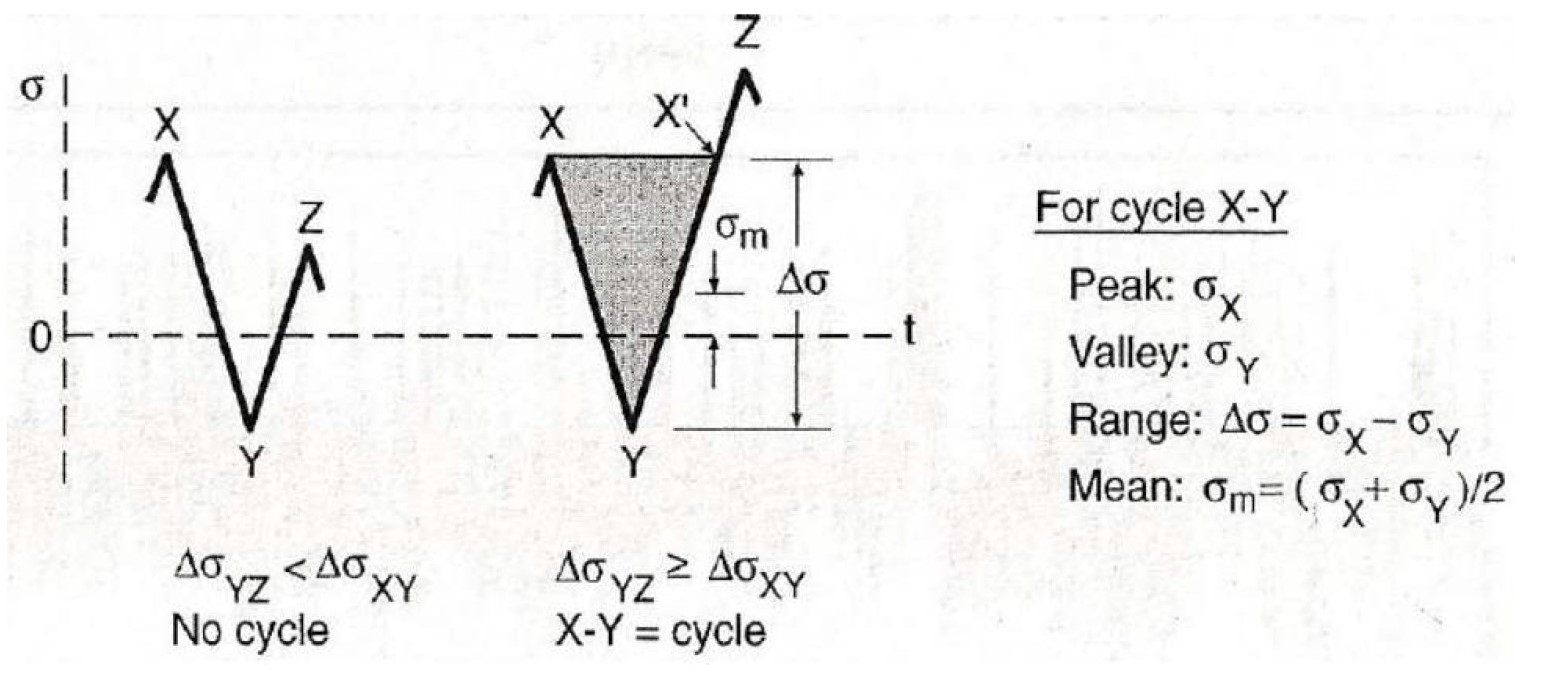
\includegraphics[width=0.7\linewidth, trim = {0mm 0mm 0mm 0mm} , clip]{felipe/fig_felipe/rain_flow_2.jpg}
    \caption{Definição matemática formal do método de identificação.}
    \label{rain_flow_2}
\end{figure}

Como o método só lida com ciclos de tensão, o primeiro passo nesta análise é excluir da série todos os pontos que não são picos nem vales. Como se assume que este ciclo de carregamento será aplicado de forma contínua e periódica, não faz diferença o ponto de início da análise se os pontos anteriores a este forem transpostos para o final da série temporal de tensões. Assim, inicia-se o método no máximo valor de tensão da série. Isso é feito para evitar problemas com o método de contagem. Além disto repete-se o primeiro ponto (máximo global) no final da série, também para fins de tornar a série amigável ao algorítmo de contagem, sem comprometimentos quanto à acurácia da contagem.

Após a adequação, o algorítimo passará pelos seguintes passos a partir do primeiro elemento da série:
\begin{itemize}
    \item É executada a análise \emph{Rainflow} de três pontos ($X_i$ , $X_{i+1}$ e $X_{i+2}$);
    \item Se identificado um ciclo de carregamento, são armazenados os dados do ciclo ( $\sigma_{m}$ , $\sigma_{a}$ ) e se exclui da análise os dois primeiro pontos ($X_i$ e $X_{i+1}$). Depois disso, o algorítmo é encaminhado para o primeiro elemento da série temporal;
    \item Se não for identificado um ciclo de carregamento a análise é levada ao próximo passo de tempo e se repete este protocolo;    
\end{itemize}

Dessa forma este protocolo se repete até o momento em que sobrar apenas dois pontos, o inicial e o final, momento em que o algorítmo se encerra.
 
As informações que se tira de cada ciclo de tensão identificado são $\sigma_{a}$ e $\sigma_{m}$ que podem ser definidos como:

\begin{equation}\label{eq.1}
    \sigma_a = \left| \frac{\sigma_{i} - \sigma_{i+2}}{2} \right|,
\end{equation}

\begin{equation}\label{eq.2}
    \sigma_m = \frac{\sigma_{i} + \sigma_{i+2}}{2}.
\end{equation}

\subsection{Método de Goodman modificado}

Com o método de Goodman modificado somos capazes de determinar uma tensão alternada equivalente $\sigma_{ar}$, onde o efeito de tensão média $\sigma_{m}$ é levado em conta. Assim, a partir disto determina-se a curva de tensão versus número de ciclos (S-N) que pode ser utilizada para o cálculo da vida em fadiga.

Assim, $\sigma_{ar}$ pode ser comparado diretamente com $\sigma_{a}$ (calculado na Eq.\ref{eq.2}) ao se considerar $R = -1$. Pode-se determinar $\sigma_{ar}$ com o método de Goodman modificado, como descrito em \cite{dowling2007}:

\begin{equation}
    \sigma_{ar} = \frac{\sigma_a}{1 - \frac{\sigma_m}{\sigma_f^\prime}},
\end{equation}

onde $\sigma_f^\prime$ é uma tensão ajustada com base na curva S-N para $\sigma_m = 0$, sendo específica para cada material e constante. Para se chegar a esse valor utiliza-se da seguinte relação:

\begin{equation}
    \sigma_a = \sigma_f^\prime \left( 2 N_f \right)^{b},
\end{equation}

onde $b$ também é encontrado a partir da curva S-N e é única e constante para cada geometria e $N_f$ denota o número de ciclos para a falha do material.

Dessa forma, para determinar este valor, por fim, utiliza-se a seguinte expressão:


\begin{equation}
    N_f = \frac{1}{2} \left( \frac{\sigma_{ar}}{\sigma_f^\prime}  \right)^{1/b}.
\end{equation}

Dessa forma, a partir dos dados  de fadiga coletados do algorítmo \emph{Rainflow} e de dados do material e da geometria, se tem tudo que é necessário para o desenvolvimento da vida em fadiga a partir do método de Goodman modificado. Para isso, derivam-se as expressões nos seguintes equacionamentos:

\begin{equation}
    N_f = \frac{1}{2} \left( \frac{\sigma_a}{\sigma^\prime_f - \sigma_m } \right)^{1/b}
\end{equation}

\begin{equation}
    B_f = \frac{1}{\sum \frac{1}{N_f}}
\end{equation}

Onde $B_f$ representa a vida em fadiga do material quando exposto à série  temporal de tensão utilizada na análise \emph{Rainflow}

\subsection{Método KPLS de predição de séries temporais}

O modelo KPLS (Kriging by partial least squares) é bem mais rápido que Kriging clássicos por lidar com um menor número de hiperparâmetros. Além disso ele apresenta boa performance em problemas multidimensionais. 

O equacionamento principal deste método pode ser observado na Eq.\ref{kpls}:
    
\begin{equation}\label{kpls}
    \prod^{nx}_{l=1} \prod^{nx}_{k=1} \text{exp} \left( -\theta_l(w_l^{(k)} x_l^{(i)} - w_l^{(k)} x_l^{(j)} )^2\right).
\end{equation}

O método foi aplicado a partir do pacote SMT \cite{BOUHLEL2019}.

\section{Resultados}

Neste segmento se falará dos resultados obtidos a partir dos códigos desenvolvidos em cada etapa desta pesquisa, começando com uma amostragem dos dados de tensão. Segue-se então para os resultados de vida em fadiga calculados para todos os elementos estruturais do \emph{riser}. Em seguida mostra-se o resultado de uma predição da série feita com a metodologia KPLS, com erros estatísticos associados. Mostram-se então os gráficos de vida em fadiga advindos destas séries parcialmente preditas, concluindo-se com análise dos erros.

\subsection{Estudos introdutórios}

De início aplicou-se o \emph{Rainflow} nos resultados da simulação do Anflex. Se configurou o programa para que armazenasse em memória a tensão externa de Von Mises de cada elemento estrutural para cada passo de tempo. O resultado de uma hora de simulação foram séries temporais de $18000$ passos para cada elemento estrutural. A unidade de medida das tensões era $kPa$ e o passo de tempo era de $0.2 s$. Na Fig.\ref{serie_temporal} podemos observar uma destas séries:

\begin{figure}[!ht]
    \centering
    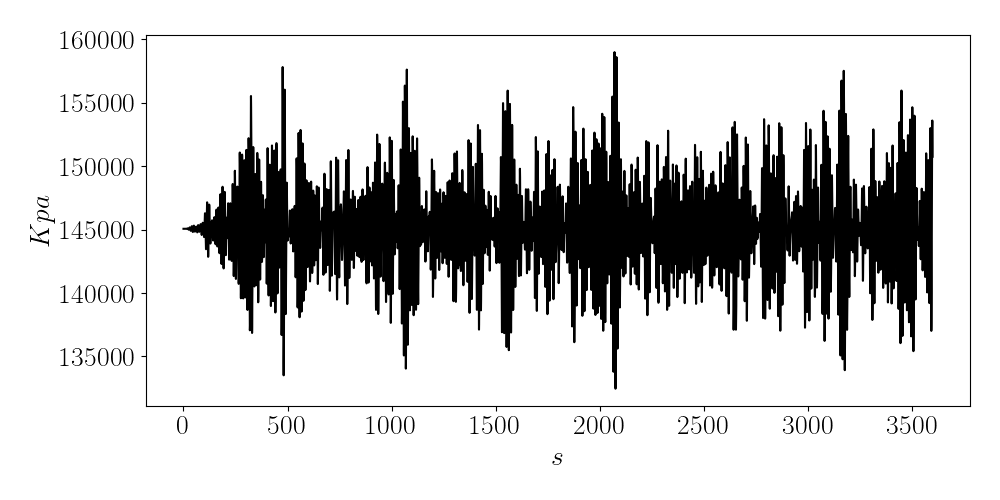
\includegraphics[width=0.96\linewidth, trim = {0mm 0mm 0mm 0mm} , clip]{felipe/fig_felipe/tensao_tempo.png}
    \caption{Série temporal de tensões externas de Von Mises do elemento \emph{PP\_M0520212}. }
    \label{serie_temporal}
\end{figure}

A partir das séries de tensão foi possível calcular as vidas em fadiga de cada elemento com o método \emph{Rainflow} depois de se tratar os dados como descrito em \ref{rainflow}. O resultado pode ser visto adiante, junto de dados estatísticos:

\begin{figure}[!ht]
    \centering
    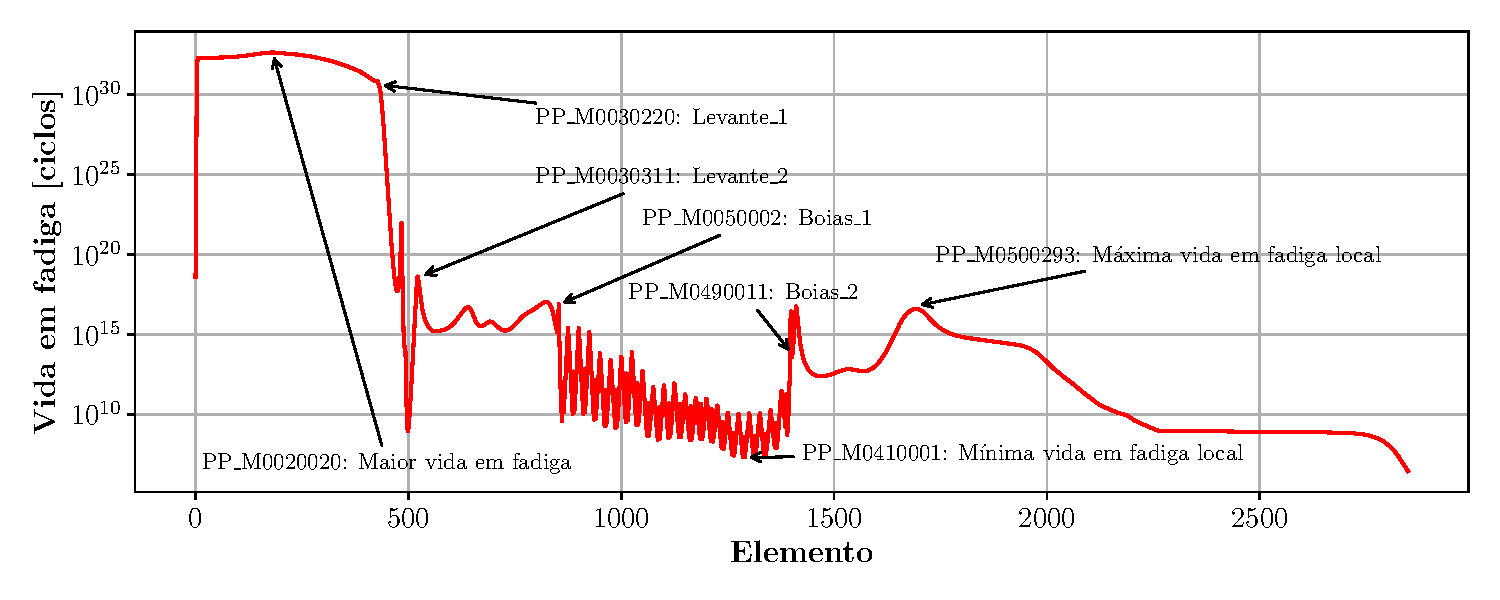
\includegraphics[width=\linewidth, trim = {0mm 0mm 0mm 0mm} , clip]{felipe/fig_felipe/Vida_em_fadiga_series_1.pdf} 
    \caption{Vida em fadiga para cada elemento estrutural do \emph{riser} simulado no Anflex. }
    \label{vida_em_fadiga}
\end{figure}

Observam-se bons resultados, sendo possível relacionar vários pontos no gráfico com as estruturas reais do \emph{riser} em configuração \emph{lazy-wave}.

\begin{figure}[!ht]
    \centering
    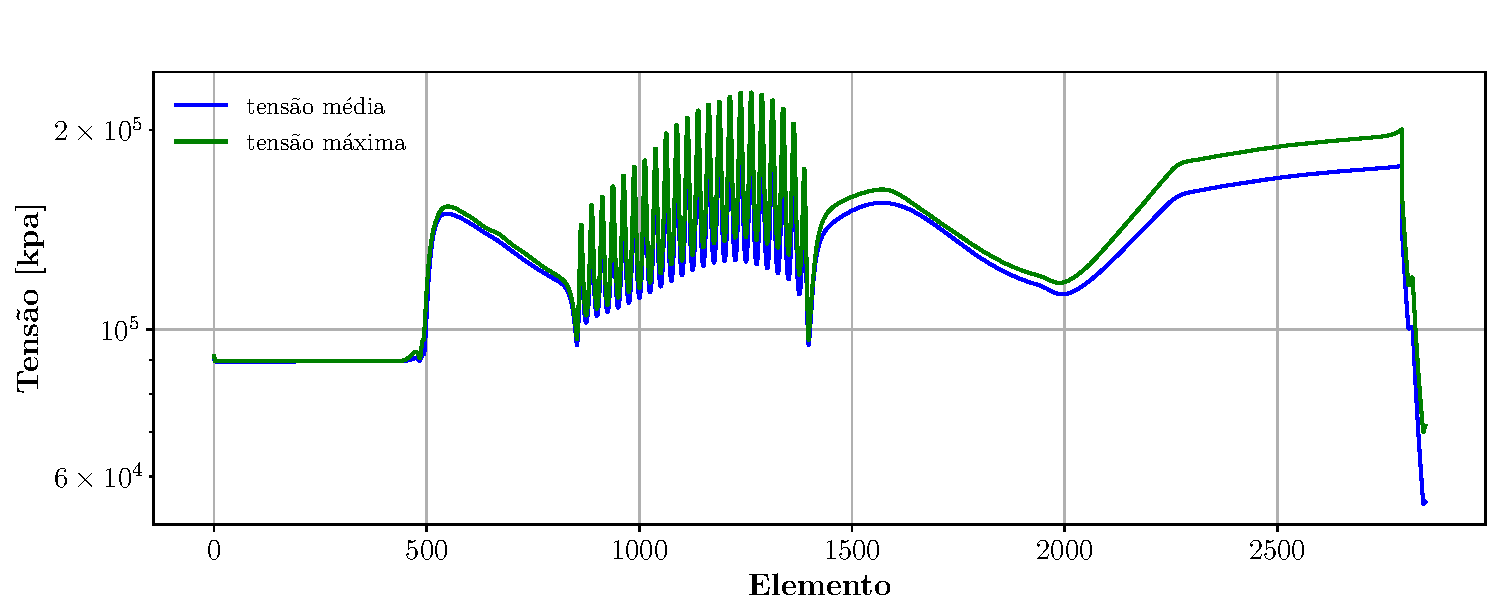
\includegraphics[width=\linewidth, trim = {0mm 0mm 0mm 0mm} , clip]{felipe/fig_felipe/Vida_em_fadiga_series_2.pdf} 
    \caption{Dados estatísticos das séries temporais de cada elemento estrutural. }
    \label{vida_em_fadiga_estatistica}
\end{figure}

Na Fig.\ref{vida_em_fadiga_estatistica} pode-se observar uma anomalia nos últimos elementos estruturais do \emph{riser}. Isso pode ser explicado pelo fato de que estes elementos fazem parte do acoplamento entre a estrutura estudada e o corpo rígido flutuante. Dessa forma, suas propriedades mecânicas são diferentes e não carregam representatividade física.

\subsection{Resultados preliminares do método KPLS}

Utilizaram-se os dados de rotação e deslocamento do ponto de ancoragem (elemento \emph{PP}) como entrada para o treino do modelo. Tem-se a predição de metade da série, isto é, foram utilizados 9000 passos para treino, prevendo-se o restante (50\%). O resultado obtido pode ser visto adiante:

\begin{figure}[!ht]
    \centering
    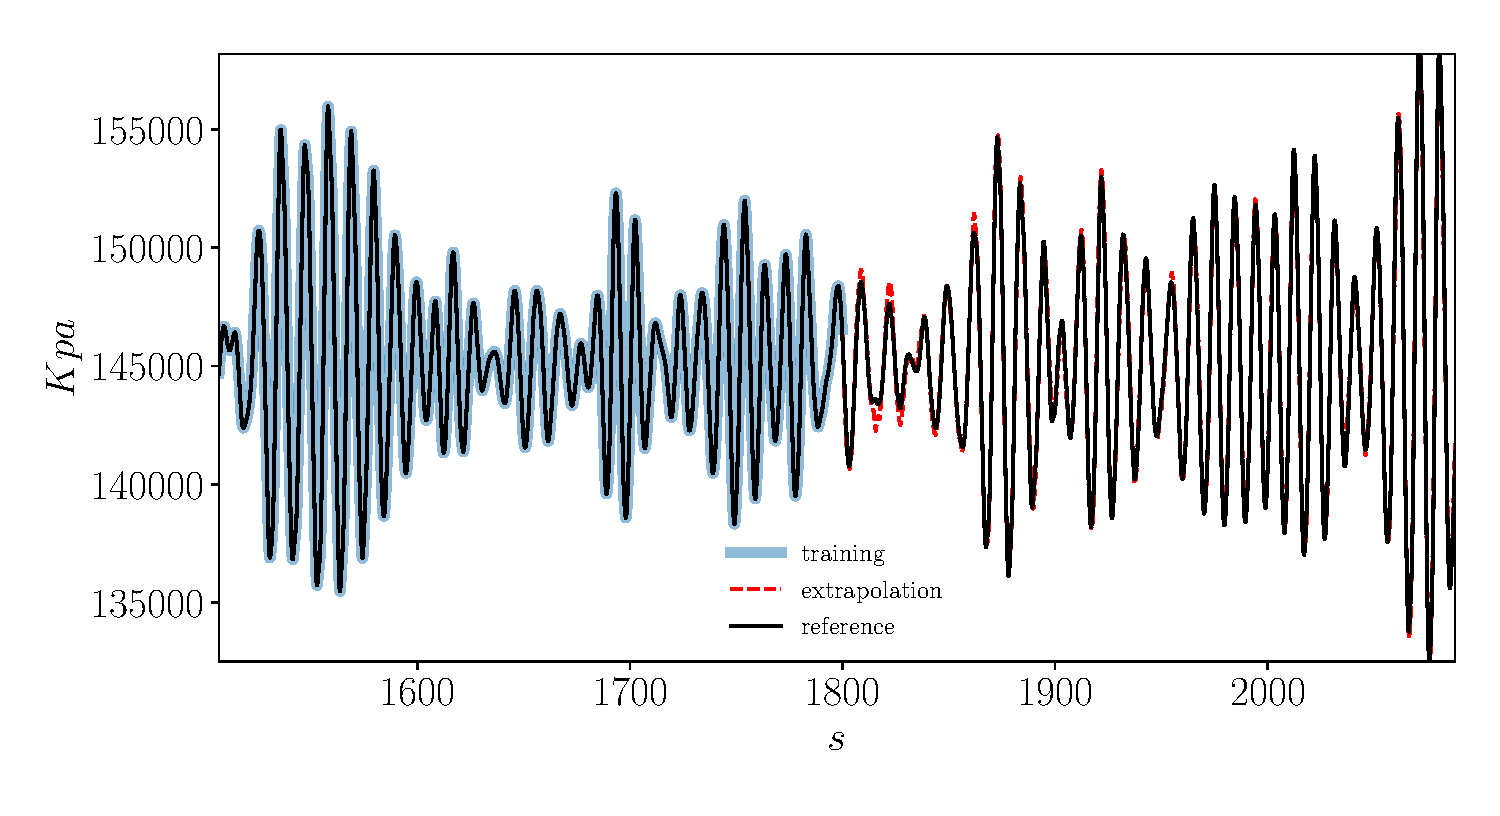
\includegraphics[width=1\linewidth, trim = {0mm 0mm 0mm 0mm} , clip]{felipe/fig_felipe/tensao_tempo_predicted_1.pdf} 
    \caption{Recorte da série temporal de tensões externas de Von Mises do elemento \emph{PP\_M0520212}. Com demonstração da extrapolação feita a partir do método \emph{KPLS}.}
    \label{serie_tensao_predicted_1}
\end{figure}

No caso exposto na Fig.\ref{serie_tensao_predicted_1}, observou-se uma média dos erros de $130.59 kPa$, que resulta em um desvio percentual de $0.09\%$ quando comparado ao valor médio da série de tensões. O erro por raiz da média dos quadrados das diferenças (norma L2, que denota o erro por desvio padrão) foi de $231.28 kPa$. Somente $0.16\%$ do valor médio da série temporal de tensões. O maior erro observado em toda a série foi de $1321.2 kPa$, que corresponde a somente $0.91\%$ do valor médio da série temporal.

Os dados das séries temporais de tensões expostas na Fig.\ref{serie_tensao_predicted_1} foram então analisadas com o método \emph{Rainflow} e Goodman modificado para o desenvolvimento das vidas em fadiga. Os resultados foram $5772770299$ ciclos de vida para a série de referência e $6143567360$ para a parcialmente predita, o que resultou em um erro percentual de $6.42\%$.

\subsection{Resultados gerais de vida em fadiga para séries feitas via KPLS}

Dessa forma, a análise foi feita para diferentes porcentagens de passos de tempo dedicados para treino ( $10\%$ , $20\%$ , $30\%$ , $40\%$ e $50\%$), sendo o restantes dos pontos conseguidos a partir do método KPLS. Além disso o estudo foi feito em todos os elemento estruturais do \emph{riser}.

\begin{figure}[!ht]
    \centering
    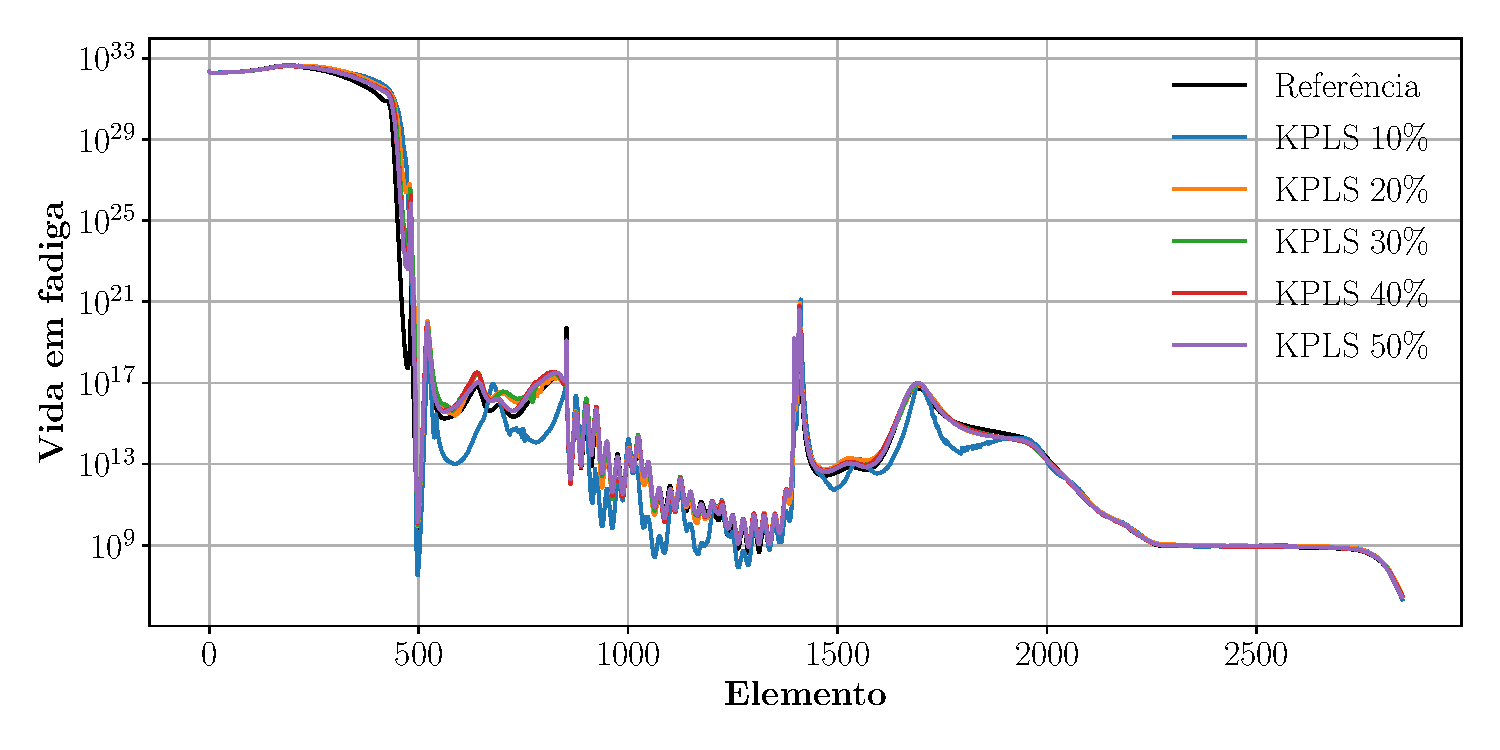
\includegraphics[width=1\linewidth, trim = {0mm 0mm 0mm 0mm} , clip]{felipe/fig_felipe/vida_fadiga_comparation.pdf} 
    \caption{Resultados de vida em fadiga calculados para cada elemento estrutural do \emph{riser}, para cada porcentagem de passos de tempo dedicados ao treino do modelo.}
    \label{comparation}
\end{figure}

Assim, notou-se que conforme se aumenta a porcentagem do número de passos de tempo dedicados ao treino observa-se uma diminuição no erro. Fez-se um estudo estatístico sobre estes resultados, com erros associados a cada porcentagem de treinamento. O resultado pode ser conferido adiante:


\begin{figure}[!ht]
    \centering
    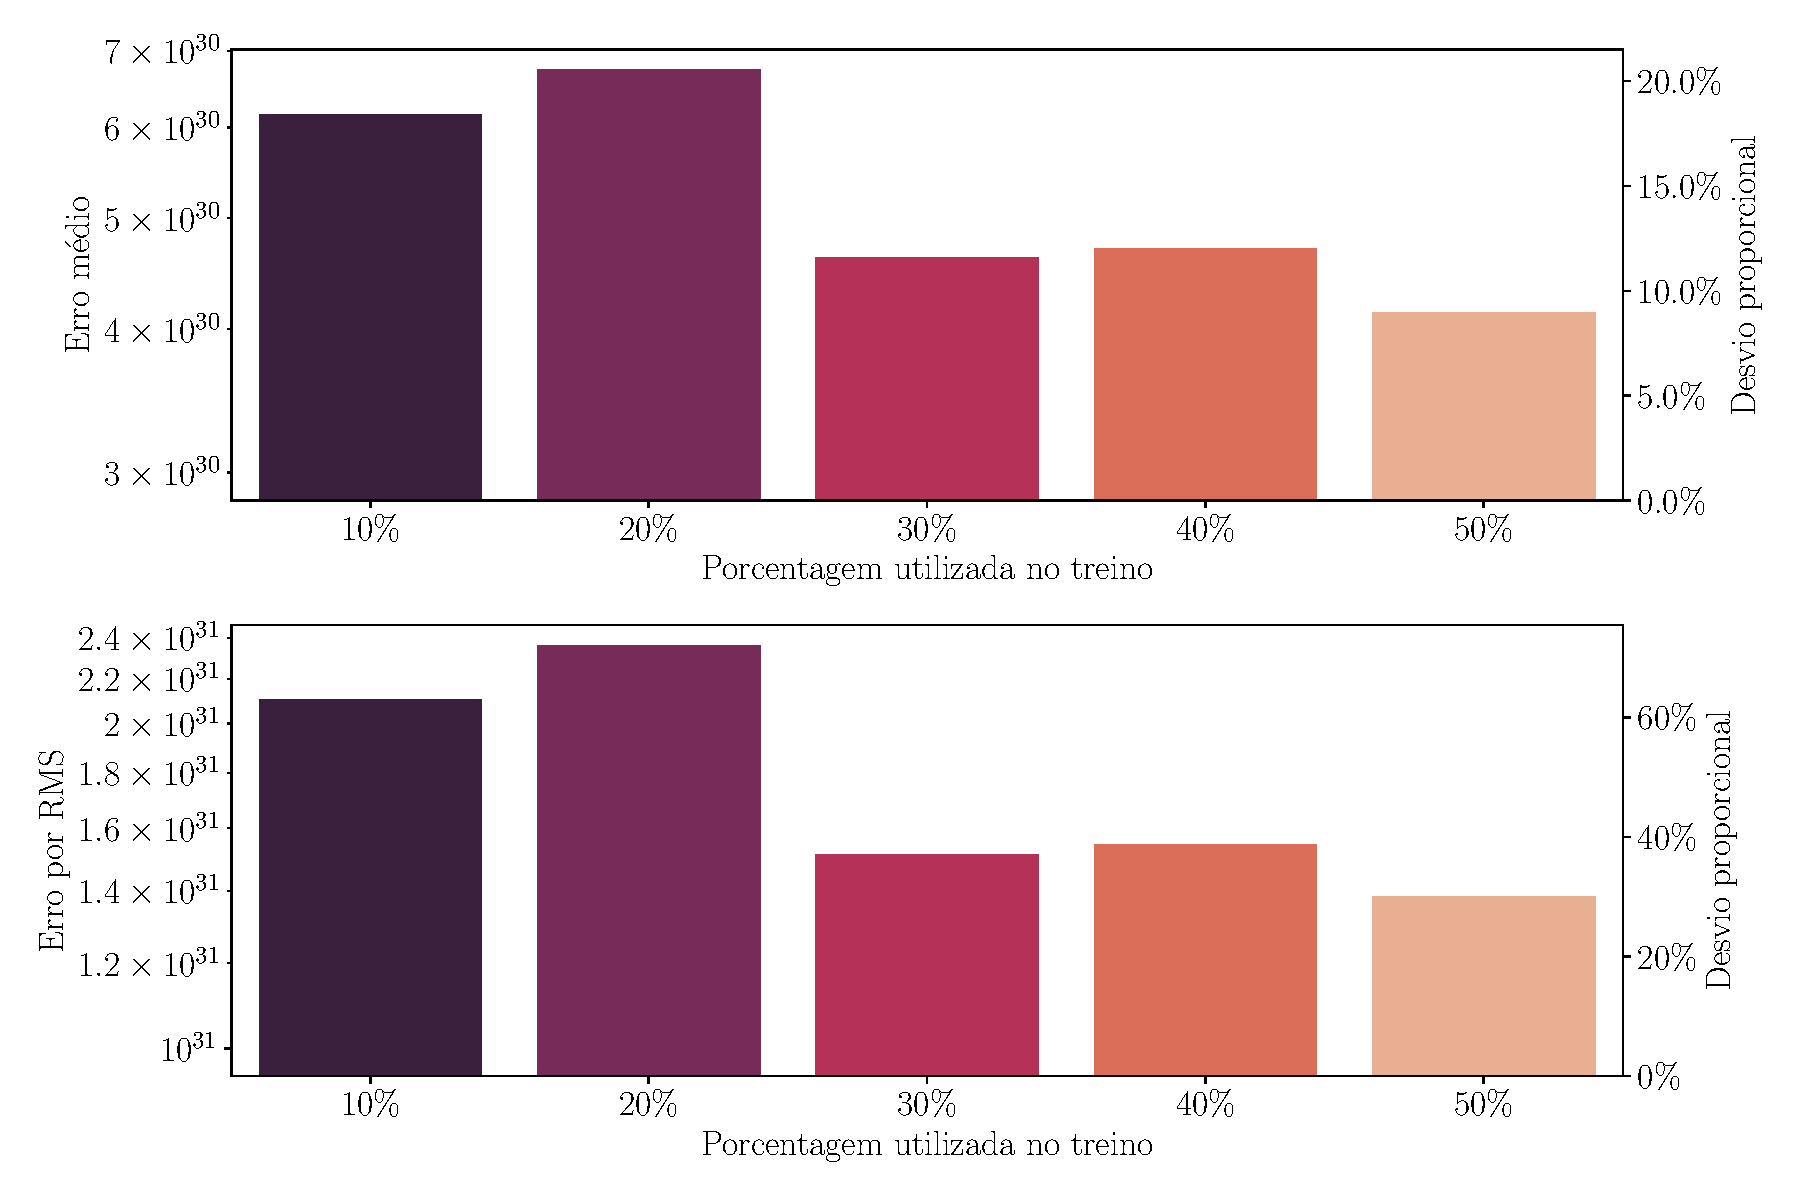
\includegraphics[width=1\linewidth, trim = {0mm 0mm 0mm 0mm} , clip]{felipe/fig_felipe/fadiga_estatisticas.pdf} 
    \caption{Dados estatísticos dos resultados obtidos quanto a vida em fadiga. Com a média dos erros e desvio padrão. Também adimensionalizados ao serem divididos pelo valor médio de ciclos da vida em fadiga.}
    \label{estatistica_valores}
\end{figure}

Notaram-se erros que tendem a diminuir com o aumento da porcentagem de passos para treinamento. Com desvios percentuais significativos e de tendência não linear.

As séries temporais de tensão parcialmente preditas também foram analisadas e os resultados estatísticos também podem ser vistos em Fig.\ref{L1_comparation}, Fig.\ref{L2_comparation} 3 Fig.\ref{Li_comparation}. Nelas tonam-se mais regularidades quanto às manifestações da alterações de número de passos de tempo dedicados ao treino do KPLS. Também observa-se que a maior quantidade de erros encontram-se próximos à estrutura flutuante do \emph{riser} e próximos do local onde o objeto de estudo toca o leito do mar, algo que pode ser explicado pela complexidade envolvida nestes segmentos.

\begin{figure}[!ht]
    \centering
    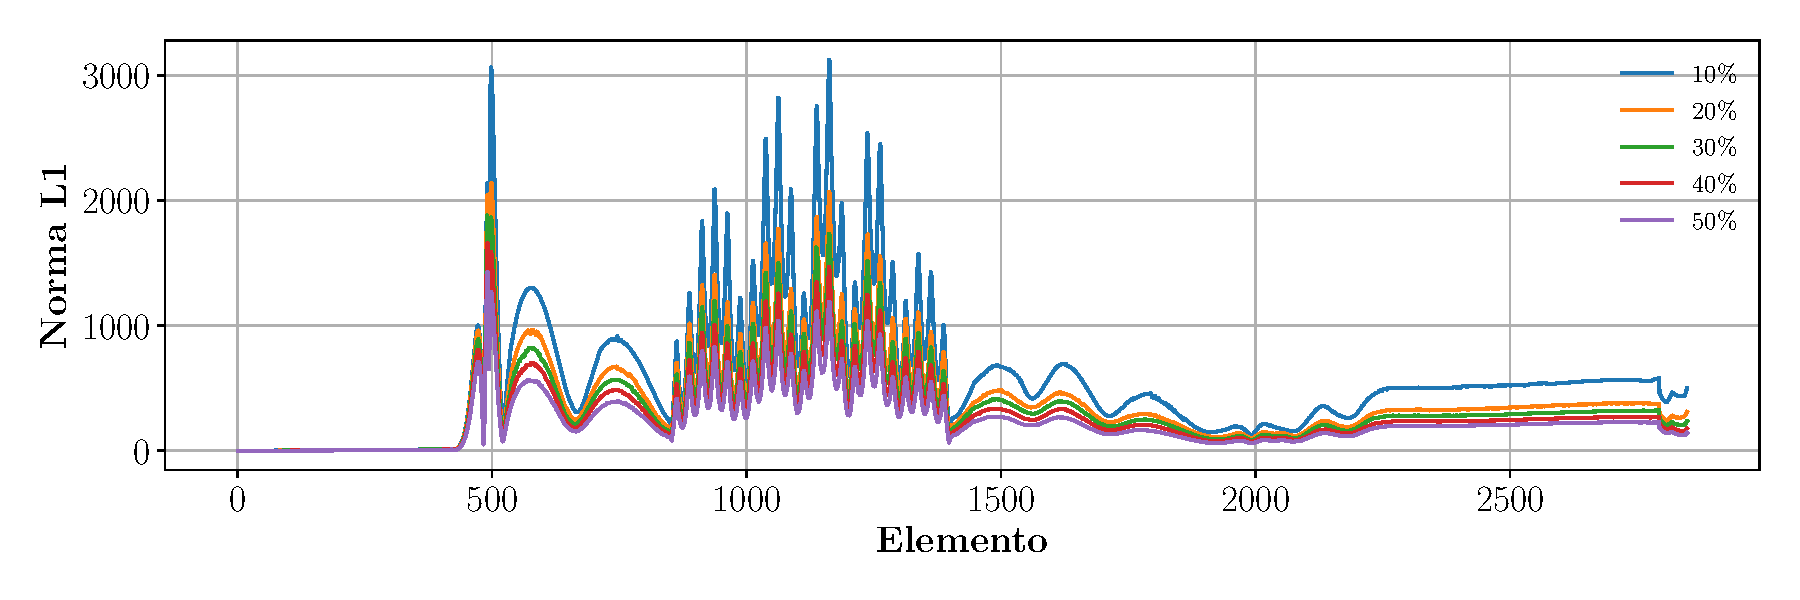
\includegraphics[width=0.95\linewidth, trim = {0mm 0mm 0mm 0mm} , clip]{felipe/fig_felipe/L1_comparation.pdf} 
    \caption{Análise da média dos erros das séries temporais devido à aplicação do método KPLS de predição.}
    \label{L1_comparation}
\end{figure}

\begin{figure}[!ht]
    \centering
    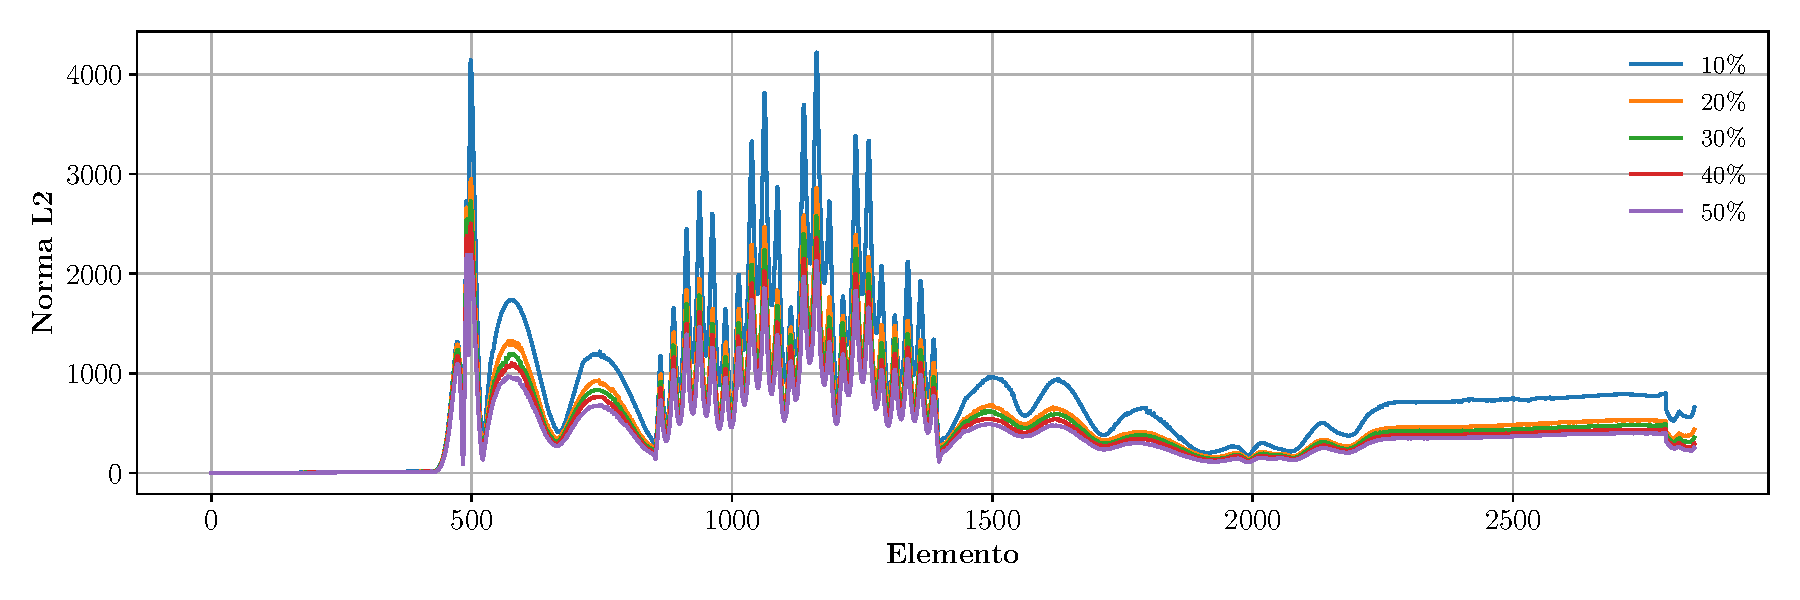
\includegraphics[width=0.95\linewidth, trim = {0mm 0mm 0mm 0mm} , clip]{felipe/fig_felipe/L2_comparation.pdf} 
    \caption{Análise por RMS dos erros das séries temporais devido à aplicação do método KPLS de predição.}
    \label{L2_comparation}
\end{figure}

\begin{figure}[!ht]
    \centering
    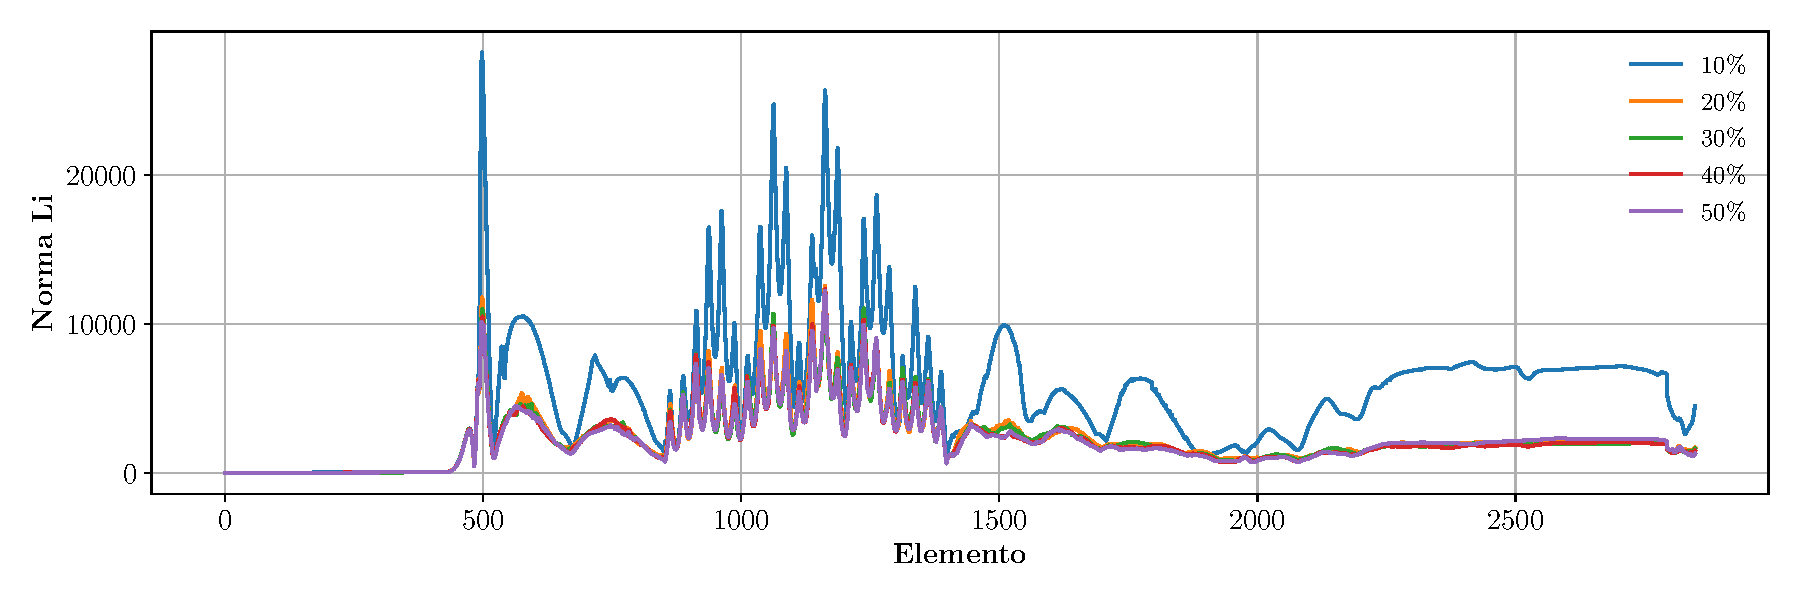
\includegraphics[width=0.95\linewidth, trim = {0mm 0mm 0mm 0mm} , clip]{felipe/fig_felipe/Li_comparation.pdf} 
    \caption{Análise dos maiores erros das séries temporais devido à aplicação do método KPLS de predição.}
    \label{Li_comparation}
\end{figure}


\section{Conclusão}

Conclui-se que o método KPLS para predição de séries temporais é aplicável no desenvolvimento de vida em fadiga ao se levar em conta quanto de erro é admissível no caso estudado. Isso pode causar grande otimização no processo uma vez que reduz de forma significativa o tempo de simulação necessário para o desenvolvimento da análise sem grandes comprometimentos quanto à acurácia do método numérico. 

Vale ressaltar que a decisão de aplicação da metodologia KPLS também depende do tipo de análise que será feita, uma vez que a predição causa desvios significativos dependendo do segmento do \emph{riser}, como nos entornos de zonas flutuantes e nos pontos de contato das estruturas com o leito marinho. Assim, pontos sujeitos a grandes não linearidades dinâmicas resultam em anomalias perceptíveis. 

No futuro deste estudo pretende-se analisar mais porcentagens de traino para o método KPLS, além de se procurar outros casos para se aplicar esta análise.
